
\newcommand{\castpatternsection}[1]{\noindent\textbf{#1.}}
\newcommand{\pname}[1]{\textsc{#1}}
\newcommand{\group}[1]{\subsection*{#1 Patterns}}

\newenvironment{pattern}[1]{
	\newcommand{\desc}{\castpatternsection{Description}}
	\newcommand{\instances}{\castpatternsection{Instances}}
	\newcommand{\detection}{\castpatternsection{Detection}}
	\newcommand{\discussion}{\castpatternsection{Discussion}}
	\newcommand{\related}{\castpatternsection{Related Patterns}}
    \newcommand{\thisp}{\textsc{#1}}
    \subsection{\pname{#1}}
    \label{pat:#1}
	\desc
}{}

\chapter{Casting Operations in the Wild}
\label{cha:casts}

Casting operations provide the means to escape the static type system.
\emph{But do they pose a problem for developers?}
Several studies
\citep{kechagiaUndocumentedUncheckedExceptions2014,coelhoUnveilingExceptionHandling2015,zhitnitskyTop10Exception2016}
show that \code{ClassCastException} is in top 10 of exceptions being
thrown when analysing stack traces.

To illustrate the sort of problem developers have when applying casting
conversions, we performed a simple search for commits and issues
including the term \code{ClassCastException} on \github{}
within projects marked as using the \java{} language.
The search returns about
$171K$\footnote{\url{https://github.com/search?l=Java&q=ClassCastException&type=Commits}}
and
$73K$\footnote{\url{https://github.com/search?l=Java&q=ClassCastException&type=Issues}}
results respectively at the time of writing.
At first glance, these results indicate that indeed
\code{ClassCastException} represents a source for
problems to developers.
We have included here a few commit results as an example.%
\footnote{To easily spot what the developer has changed to fix
the \code{ClassCastException}, we present each source code excerpt
using the Git commit \emph{diff} as reported by \github{}.}

\textbf{Forgotten Guard.}
The following listing%
\footnote{\url{https://github.com/jenkinsci/extra-columns-plugin/commit/02d10bd1fcbb2e656da9b1b4ec54208b0cc1cbb2}}
shows a cast applied to the variable \code{job} (in line $6$)
that throws \code{ClassCastException} because the developer forgot to include a guard.
In this case, the developer fixed the error by introducing a guard on the cast with \code{instanceof}.

\begin{lstlisting}[style=java]
@@ -41,6 +41,8 @@ public SCMTypeColumn() {
   }
       public String getScmType(@SuppressWarnings("rawtypes") Job job) {
+        if(!(job instanceof AbstractProject<?, ?>))
+            return "";
       AbstractProject<?, ?> project = (AbstractProject<?, ?>) job;
       return project.getScm().getDescriptor().getDisplayName();
   }
\end{lstlisting}

\textbf{Wrong Cast Target.}
In the next example%
\footnote{\url{https://github.com/GoldenGnu/jeveassets/commit/5f4750bc8cfa7eed8ad01efd8add2cd2cc9bd831}}
the \code{CustomFileFilter} is an inner static class inside \code{JCustomFileFilter}.
Notice the cast happens inside an \code{equals} method, where this idiom is well known.
But the developer has used the outer --- wrong --- class to cast to.

\begin{lstlisting}[style=java]
@@ -156,7 +156,7 @@ public boolean equals(Object obj) {
  if (getClass() != obj.getClass()) {
      return false;
  }
- final JCustomFileChooser other = (JCustomFileChooser) obj;
+ final CustomFileFilter other = (CustomFileFilter) obj;
  if (!Objects.equals(this.extensions, other.extensions)) {
      return false;
  }
\end{lstlisting}

\textbf{Generic Type Inference Mismatch.}
In the following listing,%
\footnote{\url{https://github.com/ethereum/ethereumj/commit/224e65b9b4ddcb46198a6f8faf69edc65d34d382}}
the \emph{dynamic} property \code{"peer.p2p.pingInterval"}
(lines $5$ and $6$) has type \code{int}.
To fix the error, the developer only changed the type of the
literal $5$: from \code{long} to \code{int}.

\begin{lstlisting}[style=java]
@@ -281,7 +281,7 @@ private void startTimers() {
        } catch (Throwable t) {
            logger.error("Unhandled exception", t);
        }
-   }, 2, config.getProperty("peer.p2p.pingInterval", 5L), TimeUnit.SECONDS);
+   }, 2, config.getProperty("peer.p2p.pingInterval", 5), TimeUnit.SECONDS);
}
\end{lstlisting}

Looking at the definition of the \code{getProperty} method below,%
\footnote{\url{https://github.com/ethereum/ethereumj/blob/224e65b9b4ddcb46198a6f8faf69edc65d34d382/ethereumj-core/src/main/java/org/ethereum/config/SystemProperties.java\#L312}}
it obtains a dynamic property given a property name.
If it finds a value, return it.
Otherwise, returns the default value (second argument).
But the return type of \code{getProperty} is a generic type inferred
by the type of the default value, in this case, \code{long}.
The \code{ClassCastException} is then thrown in line $5$,
when casting \code{java.lang.Integer} to \code{java.lang.Long}.
To then fix the bug, the developer changed the type of the literal:
from \code{long} to \code{int}.

\begin{lstlisting}[style=java]
public <T> T getProperty(String propName, T defaultValue) {
    if (!config.hasPath(propName)) return defaultValue;
    String string = config.getString(propName);
    if (string.trim().isEmpty()) return defaultValue;
    return (T) config.getAnyRef(propName);
}
\end{lstlisting}

% \textbf{Compiler Bug}
% One issue\footnote{\url{https://github.com/mockito/mockito/issues/357}} 
% shows bad things happen when abusing the type system.
% A bug in the \emph{javac} compiler\footnote{\url{https://bugs.openjdk.java.net/browse/JDK-8058199}}
% was causing \code{checkcast}\footnote{\url{https://docs.oracle.com/javase/specs/jvms/se8/html/jvms-6.html\#jvms-6.5.checkcast}}
% instructions to be skipped.
% This bug was fixed in JDK 9, breaking Mockito answer strategies.

This indicates that casts represents a source of errors for developers.
We present here our partial results for the cast study.
First we give an overview of the study in \S\ref{sec:casts:overview},
while \S\ref{sec:casts:stats} gives an estimation of how often a cast operator is used.
Finally, \S\ref{sec:casts:methodology} introduces the methodology we plan to use to discover cast usage patterns.

\section{Overview of our Study}
\label{sec:casts:overview}

We propose to answer the following question:
\emph{How and when do developers need to escape the type system?}
The cast operator in \java{} provides the means to view a reference at a different type as it was declared.
Upcasts conversions are done automatically by the compiler.
% DONE: Removed
% Nevertheless, in some situations a developer is forced to insert upcasts.
In the case of downcasts, a check is inserted at run-time to verify that the conversion is sound, thus escaping the type system.
\emph{Why is so?}
Therefore, we believe we should care about how the casting operations are used in the wild.
Specifically, we want to answer the following research questions:

\begin{enumerate}[label=$CRQ\arabic*:$,ref=$CRQ\arabic*$,leftmargin=3.4\parindent]
\item\label{enum:rq1}{\bf \crqA}
We want to understand to what extent application code actually uses casting operations.
\item\label{enum:rq2}{\bf \crqB}
If casts are actually used in application code, we want to know how and why developers need to escape the type system.
\item\label{enum:rq3}{\bf \crqC}
In addition to understand how and why casts are used, we want to measure how often developers need to resort to certain idioms to solve a particular problem.
\end{enumerate}

To answer the above questions,
we need to determine whether and how casting operations are actually used in
real-world \java{} applications.
To achieve our goal, several elements are needed.

\textbf{Source Code Analysis.}
We have implemented our study using the \ql{} query language:
``a declarative, object-oriented logic programming language for querying complex, potentially recursive data structures encoded in a relational data model''~\citep{avgustinovQLObjectorientedQueries2016}.
\ql{} allows us to analyze programs at the source code level by abstracting the code sources into a Datalog model.
Besides providing structural data for programs, \ie{}, ASTs,
\ql{} has the ability to query static types and perform data-flow analysis.
To run our \ql{} queries, we have used the service provided by Semmle.\footnote{\url{https://lgtm.com/}} 

\textbf{Projects.} 
As a code base representative of the ``real world'',
we have chosen open-source projects hosted in 
\github{},
the world-most popular source code management repository.
% , \ie{},
% \github{},
%\footnote{\url{https://github.com/}},
% \gitlab{},
%\footnote{\url{https://gitlab.com/}},
% \bitbucket{},
%\footnote{\url{https://bitbucket.org/}}.
So far, we have analyzed \nproject{} \java{} projects in \lgtm{}.
We plan to scale up our analysis to the whole \lgtm{} project database.

\textbf{Usage Pattern Detection.}
After all cast instances are found, we analyze this information to discover usage patterns.
\ql{} allows us to automatically categorize cast use cases into patterns.
This methodology is described in section~\ref{sec:casts:methodology}.

% DONE: Remove: Weird statement.
% It is common that a project exhibits more than one pattern
Our list of patterns is not exhaustive.
Due to the nature of the cast operator, some casts were uncategorized as they would need a whole program analysis, \eg{}, including libraries in the analysis.

\section{Is the Cast Operator used?}
\label{sec:casts:stats}

To answer \ref{casts:rq1} (\emph{\crqA}) we want to know how many cast instances are used in a given project.
To this end, we gather the following statistics using \ql{}.
We show them here to give an estimation of the size of the code base being analized.
% DONE: Why only 24 project? Should say this is preliminary?
As mentioned above, these results are preliminary.
We plan to scale up our analysis to the whole \lgtm{} project database.

\begin{center}
\begin{tabular}{lr}
	Description & Value\\
	\hline
	Number of Projects & \nproject \\
	Number of LOC & \nloc{} \\
	Number of Methods & \nmethod \\
	Number of Methods \emph{w/}Cast & \nmethodwithcast \\
    Number of Expressions & \nexpr \\
	\hline
    Number of Cast Expressions & \nCastExpr \\
    Number of Cast Methods & \nCastMethod \\
    Number of \code{equals} Methods & \nEqualsMethod \\
    Number of \code{instanceof} Expressions & \nInstanceOf \\
    Number of type switch & \nTypeSwitch \\
\end{tabular}
\end{center}

The \emph{Number of Methods} and \emph{Number of Methods w/Cast} values includes only methods with a body, \ie{}, not abstract, nor native.
The \emph{Number of Exprs} value show how many expressions there are in the ASTs of all source code analyzed.
Finally, the \emph{Number of Casts} value indicates how many cast expressions (subtype of \code{Expr} as defined by \ql{}) were found.

% DONE: This is why, no?: Better explained
For our study, we are interested in both upcasts and downcasts.
Thus, we \emph{exclude} primitive conversions in our study
(\S$5.1.2$, \S$5.1.3$, \S$5.1.4$, and \S$5.1.13$ from the \java{} Language Specification%
\footnote{\url{https://docs.oracle.com/javase/specs/jls/se7/html/jls-5.html}}
).
The \emph{Number of Casts} value shown above include only reference conversions.
Primitive conversions are always safe (in terms of throwing \code{ClassCastException}.
A primitive conversion happens when both the type of the expression to be casted to and
the type to cast to are primitive types.
Note that with this definition, we include in our study \emph{boxed} types.
Since boxed types are reference types (and therefore not necessarily safe)
we want to include them in our analysis.

We want to know how many cast instances there are across projects.
Thus, we have computed the ratio between methods containing
at least a cast over total number of methods --- with implementation --- in a given project.
The following chart shows this ratio for all analyzed projects:

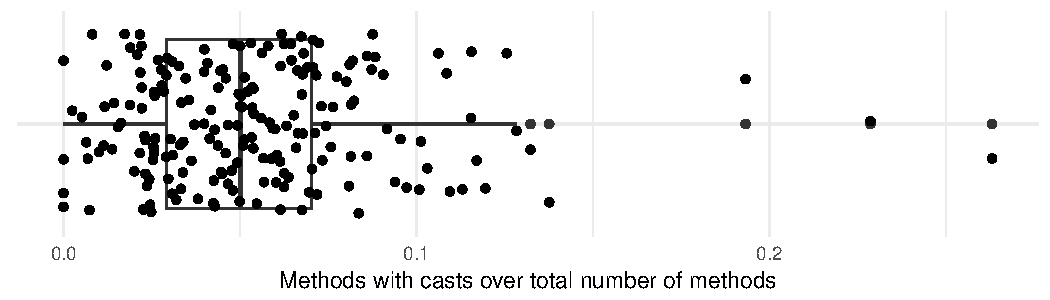
\includegraphics[width=\columnwidth,height=3.8cm]{analysis/stats-methodwcastXproject.pdf}

All projects have less than $10\%$ of methods with at least a cast.
Overall, around a~$\castpercentage{}\%$ of methods contain at least one cast operation. 
This means there is a low density of casts.
Given the fact that generics were introduced \java{} 5, this can explain this low density.

Nevertheless, casts are still used.
We want to understand why there are casts instances (\ref{casts:rq2}) and
how often the use cases that leads to casts are used (\ref{casts:rq3}).
The following sections give an answer to these questions.

% DONE: cut
% The query to gather this statistics is available online.\footnote{\url{https://gitlab.com/acuarica/java-cast-queries/blob/master/ql/stats.ql}}
% The \lang{R} script to further analyze the query results is available online as well.\footnote{\url{https://gitlab.com/acuarica/java-cast-queries/blob/master/analysis/stats.r}}

\section{Finding Casts Usage Patterns}
\label{sec:casts:methodology}

To answer both research questions
\ref{casts:rq2} (\emph{\crqB}) and \ref{casts:rq3} (\emph{\crqC})
we have used the \ql{} query language within the \lgtm{} service to look for cast instances.
%
As mentioned in section \ref{sec:casts:stats}, \ql{} treats primitive conversions as casts.
Thus, a preliminary step is to exclude them as cast instances.
The following \ql{} query shows how to retrieve all relevant cast expressions:

\begin{lstlisting}[style=ql,caption=\ql{} query to retrieve all relevant cast expressions.]
import java
from CastExpr ce where not (
ce.getExpr().getType() instanceof PrimitiveType and
ce.getTypeExpr().getType() instanceof PrimitiveType
) select ce
\end{lstlisting}

\tikzstyle{decision} = [diamond, aspect=2, draw, fill=blue!20, 
    text width=6em, text badly centered, node distance=3cm, inner sep=0pt]
\tikzstyle{block} = [rectangle, draw, fill=blue!20, 
    text width=7em, text centered, rounded corners, minimum height=2em]
\tikzstyle{block2} = [rectangle, draw, fill=blue!20, 
    text width=4.0em, text centered, rounded corners, minimum height=2em]
\tikzstyle{line} = [draw, -latex']
\tikzstyle{cloud} = [draw, ellipse,fill=red!20, node distance=3.1cm,
    minimum height=2.9em]

\begin{figure}
% \begin{wrapfigure}{r}{7.6cm}
\centering
\begin{tikzpicture}[node distance = 1.5cm, auto]
    % Place nodes
    \node [block] (run) {Run Query};
    % \node [cloud, left of=run] (tags) {Tags};
    \node [cloud, right of=run] (patterns) {Patterns};
    \node [block, below of=run] (inspect) {Inspect Casts without Pattern};
    % \node [decision, below of=inspect, node distance=1.6cm] (tag) {New Tag?};
    \node [decision, below of=inspect, node distance=2.0cm] (pattern) {New Pattern?};
    % \node [block2, left of=tag, node distance=3.1cm] (update-tags) {Update Tags};
    \node [block2, right of=pattern, node distance=3.1cm] (update-pattern) {Update Patterns};
    % \node [decision, below of=evaluate] (decide) {is best candidate better?};
    \node [block, below of=pattern, node distance=1.6cm] (stop) {Stop};
    % Draw edges
    \path [line] (run) -- (inspect);
    % \path [line] (inspect) -- (evaluate);
    % \path [line] (inspect) -- (tag);
    \path [line] (inspect) -- (pattern);
    % \path [line] (tag) -- node [near start] {yes} (update-tags);
    \path [line] (pattern) -- node [near start] {yes} (update-pattern);
    % \path [line] (update-tags) -- (tags);
    \path [line] (update-pattern) -- (patterns);
    % \path [line] (tag) -- node {no}(pattern);
    \path [line] (pattern) -- node {no}(stop);
    % \path [line,dashed] (tags) -- (run);
    \path [line,dashed] (patterns) -- (run);
\end{tikzpicture}
\caption{Process to discover cast tags and patterns.} \label{fig:process}
\end{figure}

Figure~\ref{fig:process} depicts our methodology.
We have used this initial result as a starting point for our analysis.
Afterwards, we select a random sample for manual inspection.
We manually inspected the mentioned casts trying to understand
why and how they were used.

By manually inspecting several casts instances,
we observe that certain characteristics appear often, \eg,
a cast in a overridden method, or a cast guarded by an \code{instanceof}.
We then \emph{tag} cast instances based on these observations.
We implement a \ql{} predicate that detects them and proceed
to refine our query with this new tag predicate.
% The table of tags is presented in table~\ref{table:tags}.
After a new tag is added, the query is run again to iterate over the new results.

% DONE: Remove randomly.
% Whenever we observe that those tags do not appear randomly,
Whenever we detect that those tags appear often,
we further inspect the source code to check that is indeed a pattern.
We have formalized the structure of each pattern as a \ql{} predicate based on those tags.
Similarly with tags, after a new pattern is added,
the query is run again to inspect the casts without pattern.
To sum up, our methodology iterates over the results until
no \emph{more} patterns can be detected.
% These patterns are presented in the following section.
The final \ql{} query is available online.%
\footnote{\url{https://gitlab.com/acuarica/java-cast-queries/blob/master/obs.ql}}


% DONE: What about patterns we can't write queries for?
\subsection*{Manual Categorization of Patterns}

Some code patterns might be too difficult to
express in terms of \ql{} queries.
This situation arises when the knowledge to determine
the pattern is outside the source code,
\eg, in configuration files or library call sites.
Thus, in those cases we can only acknowledge that a pattern exists,
but not how recurrent it is.

\section{Methodology}

As for the project selection, I have used the lgtm.com project database.
We can argue that this provide a good filter of projects,
since teams that want their code to be analyzed push their projects onto lgtm.com.
This will filter out for instance student projects from github.
There are also popular projects, e.g., gradle, neo4j, google guava,
that probably were pulled in by the Semmle people.
We need to double check with them, but if that’s the case,
we can make a good argument as for the project selection.

There is a total of $7.559$ projects, with a total 10,193,435 casts.
For each cast, I have the path within the project.
But to manually analyze them, I need to get the lgtm.com link.
This is necessary to actually see the code snippet in which the cast appear.
There are 215 projects for which I can’t get the lgtm.com link.
These 215 projects contains 1,162,583 casts.
There are also 516 projects which does not contain any cast.
Therefore the cast population from where make the sampling consists of
9,030,852 casts spread in 6,840 projects.

Now comes the question: What is an appropriate sample size?
Using this online calculator:

https://www.surveysystem.com/sscalc.htm

With standard parameters, Confidence Level=95\% and Confidence Interval=5,
I got a sample size of 384.
This seems sketchy.
My first approach was to increase the sample size arbitrarily,
e.g., 10,000 casts to manually analyze.
This can be too much effort.
But more importantly, how to come up with the patterns taxonomy?
The current list of patterns I have (using QL) does not cover all
existing patterns, i.e.,
when doing manual sample I have discovered new patterns.
After meeting with Gabriele, he suggested using saturation sampling:
0. Start with an empty list of patterns.
1. Perform a manual sample of, let’s say 384 casts.
2. For each new pattern seen, add it to the list of patterns.
3. If a new pattern is detected, go to step 1.


\section{Casts Usage Patterns}
\label{sec:patterns}

Using the methodology described in the above section,
we have devised $\npattern{}$ casts usage patterns.
Overall, these patterns cover around 
$\patpercentage\%$
with uncovered casts of
$\anypercentage\%$.

In this section we present the cast usage patterns we found.
Figure~\ref{fig:patterns} presents an overview of our patterns and their occurrences sort by most frequent.

\begin{figure}[ht!]
\centering
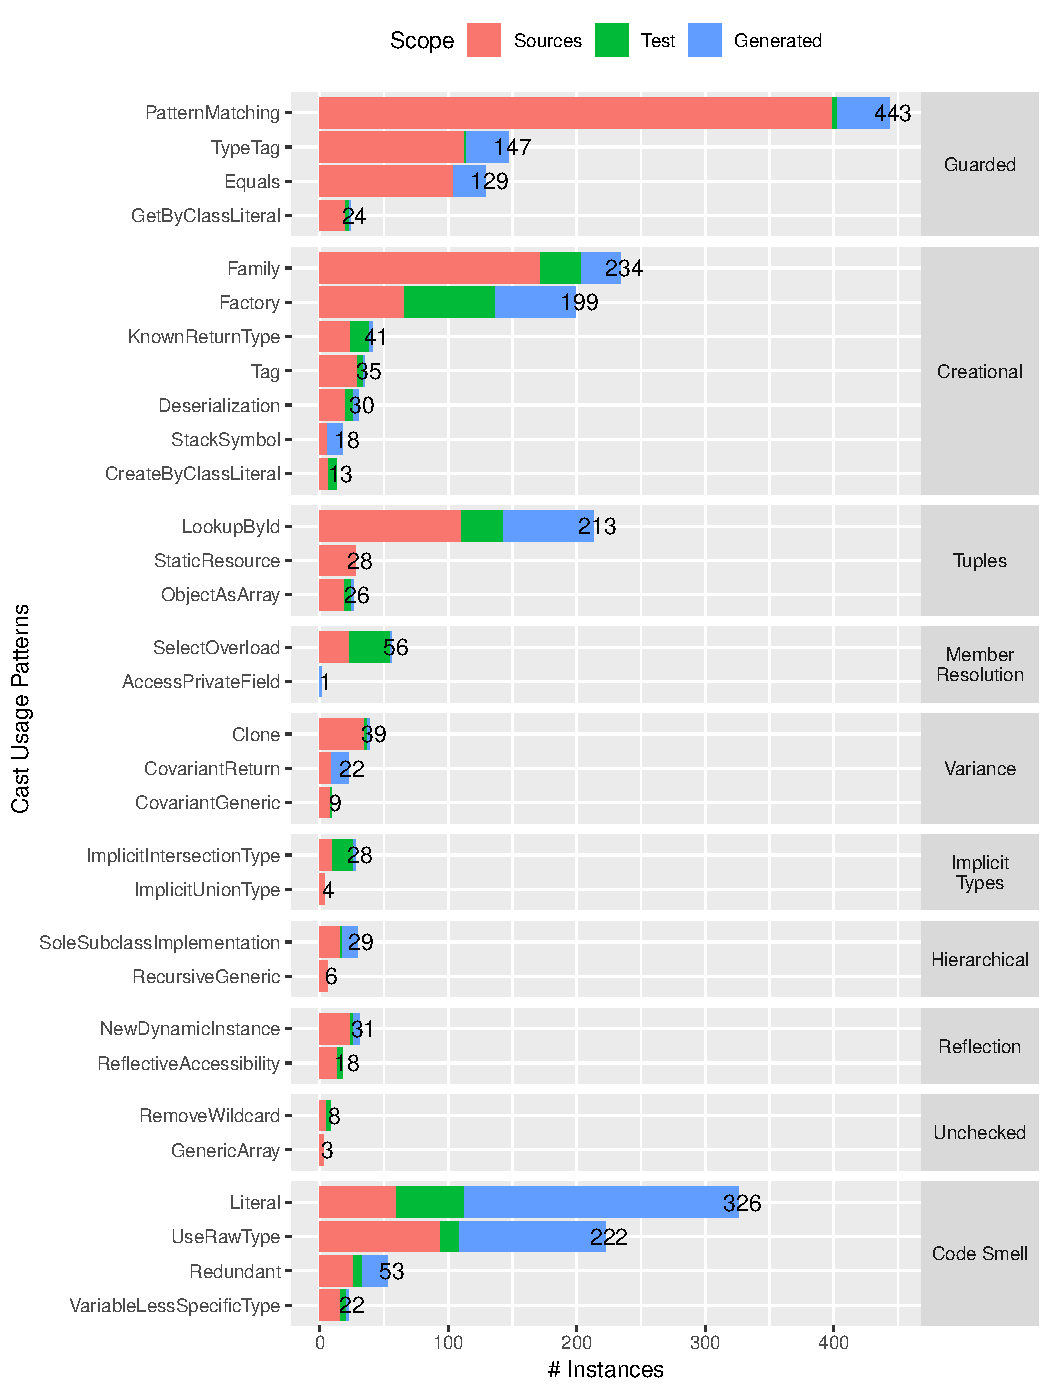
\includegraphics[width=\columnwidth]{analysis/table-patterns-5000.pdf}
\caption{Cast Patterns Occurrences} \label{fig:patterns}
\end{figure}

Any denotes all cast instances that were not categorized.
Each pattern is described using the following template:

\begin{itemize}
\item \textbf{Description.}
Tells what is this pattern about.
It gives a general overview of the structure of the pattern.
\item \textbf{Instances.}
Gives one or more concrete examples found in real code.%
\footnote{Please notice that the snippets presented here were slightly
modified for formatting purposes.
Moreover, to facilitate some snippet presentations,
we remove irrelevant code and replace it with the
comment \code{// [...]}.}
For each instance presented here,
we provide the link to the source code repository in \lgtm{}.
We provide the link in case the reader wants to do further inspection
of the snippet presented.%
\footnote{Instead of presenting \lgtm{} long URLs,
we have used the URL shortening service \url{https://bitly.com/}
for an easier reading.
}
\item \textbf{Detection.}
Describes briefly how this pattern was detected in terms of the tags
introduced in the previous section.
\item \textbf{Discussion.}
Presents suggestions, flaws, or comments about the pattern.
\item \textbf{Related Patterns.}
How the pattern being described relates to other patterns?
\end{itemize}

\group{Guarded}

\begin{pattern}{PatternMatching}
This pattern is composed of a guard (\code{instanceof}) followed by a
cast on known subtypes of the static type.
Often there is just one case and the default case, \ie,
\code{instanceof} fails, does a no-op or reports an error.
Another common approach is to have several cases,
usually one \emph{per} subtype.

\instances{}
The following listing shows an example of the \thisp{} pattern.%
\footnote{\url{http://bit.ly/2FzYYHq}}
In this example, there is only one case

% https://lgtm.com/projects/g/OpenMods/OpenBlocks/snapshot/dist-2040060754-1524814812150/files/build/sources/java/openblocks/common/tileentity/TileEntityImaginary.java?sort=name&dir=ASC&mode=heatmap#L268
\begin{minted}[highlightlines=3]{java}
Item item = helmet.getItem();
if (item instanceof ItemImaginationGlasses)
	return ((ItemImaginationGlasses)item).checkBlock(what, helmet, this);
\end{minted}

Double typecase example
\footnote{\url{http://bit.ly/2FDN9Rd}}

% https://lgtm.com/projects/g/bbossgroups/bboss/snapshot/dist-2025970729-1524814812150/files/bboss-util/src/org/frameworkset/util/ObjectUtils.java?sort=name&dir=ASC&mode=heatmap#L228
\begin{minted}[highlightlines=25]{java}
public static boolean nullSafeEquals(Object o1, Object o2) {
	if (o1 == o2) {
		return true;
	}
	if (o1 == null || o2 == null) {
		return false;
	}
	if (o1.equals(o2)) {
		return true;
	}
	if (o1.getClass().isArray() && o2.getClass().isArray()) {
		if (o1 instanceof Object[] && o2 instanceof Object[]) {
			return Arrays.equals((Object[]) o1, (Object[]) o2);
		}
		if (o1 instanceof boolean[] && o2 instanceof boolean[]) {
			return Arrays.equals((boolean[]) o1, (boolean[]) o2);
		}
		if (o1 instanceof byte[] && o2 instanceof byte[]) {
			return Arrays.equals((byte[]) o1, (byte[]) o2);
		}
		if (o1 instanceof char[] && o2 instanceof char[]) {
			return Arrays.equals((char[]) o1, (char[]) o2);
		}
		if (o1 instanceof double[] && o2 instanceof double[]) {
			return Arrays.equals((double[]) o1, (double[]) o2);
		}
		if (o1 instanceof float[] && o2 instanceof float[]) {
			return Arrays.equals((float[]) o1, (float[]) o2);
		}
		if (o1 instanceof int[] && o2 instanceof int[]) {
			return Arrays.equals((int[]) o1, (int[]) o2);
		}
		if (o1 instanceof long[] && o2 instanceof long[]) {
			return Arrays.equals((long[]) o1, (long[]) o2);
		}
		if (o1 instanceof short[] && o2 instanceof short[]) {
			return Arrays.equals((short[]) o1, (short[]) o2);
		}
	}
	return false;
}
\end{minted}


\detection{}
To detect this pattern, we look

\discussion{}
The \thisp{} pattern can be seen as an \adhoc{}
alternative to pattern matching.
This construct can be seen in several other languages, \eg,
\haskell{}, \scala{}, and \cs{}.
There is an ongoing proposal%
\footnote{\url{http://openjdk.java.net/jeps/305}} to add pattern
matching to the \java{} language.

As a workaround, alternatives to the \thisp{} pattern can be the
visitor pattern or polymorphism.
But in some cases, the chain of \code{instanceof}s is of boxed types.
Thus no polymorphism can be used.

% Maybe this should be called properly instanceof-guarded cast, to be more specific.
% This pattern checks whether a parameter in an overridden method has a more specific type.
% A cast to a variable guarded by an \code{instanceof}.
% A variable is \emph{guarded} by a condition when the condition controls
% that access to the variable, and there is no assignment after the
% condition and before the access to that variable.

The \thisp{} pattern consists of testing the runtime type of a variable against several related types.
Based on rule taken from:
It was taken from a \lgtm{} rule\footnote{\url{https://lgtm.com/rules/910065/}}.

It is a technique that allows a developer to take different actions according to the runtime type of an object.
Depending on the --- runtime --- type of an object, different cases, usually one for each type will follow.

\end{pattern}

\begin{pattern}{TypeTag}
%
\done{Matthias: Your first example doesn't have the tag in the *same* object, but passes it as a separate variable.}
%
A cast instance belonging to the \thisp{} pattern is guarded by an application-specific test instead of using an \code{instanceof} test.

\instances{}
The following example%
\footnote{\url{http://bit.ly/JesusFreke_smali_2Ho8bVL}}
shows an instance of the \thisp{} pattern.
The cast type of the parameter \code{reference} is determined by the value of the parameter \code{referenceType}.

%https://lgtm.com/projects/b/JesusFreke/smali/snapshot/dist-1306230039-1524814812150/files/dexlib2/src/main/java/org/jf/dexlib2/writer/InstructionWriter.java?sort=name&dir=ASC&mode=heatmap#L492
\begin{minted}[highlightlines=8]{java}
private int getReferenceIndex(int referenceType, Reference reference) {
    switch (referenceType) {
        case ReferenceType.FIELD:
            return fieldSection.getItemIndex((FieldRefKey) reference);
        case ReferenceType.METHOD:
            return methodSection.getItemIndex((MethodRefKey) reference);
        case ReferenceType.STRING:
            return stringSection.getItemIndex((StringRef) reference);
        case ReferenceType.TYPE:
            return typeSection.getItemIndex((TypeRef) reference);
        case ReferenceType.METHOD_PROTO:
            return protoSection.getItemIndex((ProtoRefKey) reference);
        default:
            throw new ExceptionWithContext(
                "Unknown reference type: %d",  referenceType);
    }
}
\end{minted}

In the next example,%
\footnote{\url{http://bit.ly/FenixEdu_fenixedu-academic_2SUNOUJ}}
instead of a \code{switch} statement,
an \code{if} statement is used to guard the cast (in line 6).

%https://lgtm.com/projects/g/FenixEdu/fenixedu-academic/snapshot/dist-29270029-1524814812150/files/src/main/java/org/fenixedu/academic/ui/renderers/student/curriculum/StudentCurricularPlanRenderer.java?sort=name&dir=ASC&mode=heatmap#L853
\begin{minted}[highlightlines=6]{java}
for (final IEnrolment enrolment : dismissal.getSourceIEnrolments()) {
    if (enrolment.isExternalEnrolment()) {
        generateExternalEnrolmentRow(mainTable, (ExternalEnrolment) enrolment,
                level + 1, true);
    } else {
        generateEnrolmentRow(mainTable, (Enrolment) enrolment,
                level + 1, false, true, true);
    }
}
\end{minted}

\done{Nate: Why is this not pattern matching?}
%
In the next case%
\footnote{\url{http://bit.ly/apache_poi_2FW5SXU}}
a type test is performed --- through a method call --- before actually applying the cast to the variable \code{props} (line 3).
Note that the type test is internally using the \code{instanceof} operator (line 8).
Although in this case the type test is using an \code{instanceof} operator,
it is not considered \nameref{pat:PatternMatching} because the \code{instanceof} is located in a method call.

%https://lgtm.com/projects/g/apache/poi/snapshot/dist-1790760597-1524814812150/files/src/ooxml/java/org/apache/poi/xslf/usermodel/XSLFPropertiesDelegate.java?sort=name&dir=ASC&mode=heatmap#L1367
\begin{minted}[highlightlines=3]{java}
@Override
public CTSolidColorFillProperties getSolidFill() {
    return isSetSolidFill() ? (CTSolidColorFillProperties)props : null;
}

@Override
public boolean isSetSolidFill() {
    return (props instanceof CTSolidColorFillProperties);
}
\end{minted}

In some cases, the type to be casted to is the same in every branch.
The following snippet%
\footnote{\url{http://bit.ly/loopj_android-async-http_2IpIULk}}
shows an instance of this case.
The cast is applied to the \code{message.obj} field to (line 13),
according to the value of the \code{message.what} field (line 1).
However, a similar cast is applied in the first branch (line 3).
In both branches \code{message.obj} is of type \code{Object[]},
but in the case of \code{FAILURE\_MESSAGE},
the array contains one more element (line 16).
This suggests that the \code{(Object[]) message.obj} array denotes two different objects,
but are not distinguishable from the type system perspective.

%https://lgtm.com/projects/g/loopj/android-async-http/snapshot/dist-1879340034-1549372228293/files/library/src/main/java/com/loopj/android/http/AsyncHttpResponseHandler.java?sort=name&dir=ASC&mode=heatmap#L359
\begin{minted}[highlightlines=13]{java}
switch (message.what) {
    case SUCCESS_MESSAGE:
        response = (Object[]) message.obj;
        if (response != null && response.length >= 3) {
            onSuccess((Integer) response[0], (Header[]) response[1],
                    (byte[]) response[2]);
        } else {
            AsyncHttpClient.log.e(LOG_TAG, 
                    "SUCCESS_MESSAGE didn't got enough params");
        }
        break;
    case FAILURE_MESSAGE:
        response = (Object[]) message.obj;
        if (response != null && response.length >= 4) {
            onFailure((Integer) response[0], (Header[]) response[1],
                    (byte[]) response[2], (Throwable) response[3]);
        } else {
            AsyncHttpClient.log.e(LOG_TAG,
                    "FAILURE_MESSAGE didn't got enough params");
        }
        break;
    // [...]
}
\end{minted}


\detection{}
The detection of this pattern is similar to the \nameref{pat:PatternMatching} detection, but instead of looking for an \code{instanceof} guarded cast, we look for an application-specific guard.
The guard needs to determine either the resulting type of the cast instance, or
the subsequent operations applied to the result of the cast instance if the types in every branch are the same.

\discussion{}
In some cases, the \thisp{} pattern can be replaced by \nameref{pat:PatternMatching}.
However, if the application-specific tag is a numeric value,
the \thisp{} could perform better than the \nameref{pat:PatternMatching} using \code{instanceof}.
Moreover, there are situation where the \thisp{} can not be avoid since the types to be casted to are the same.

\related{}
%
\done{Nate: PatternMatching}
This pattern is related to \nameref{pat:PatternMatching} since both denoted guarded casts.
The difference is that \thisp{} uses an application-specific test.
\nameref{pat:GetByClassLiteral} could be seen as a special case of \thisp{} where the tag is a class literal.

\end{pattern}
\begin{pattern}{Equals}
This pattern is a common pattern to implement the \code{equals} method (declared in \code{java.lang.Object}).
A cast expression is guarded by either an \code{instanceof} test or a \code{getClass} comparison (usually to the same target type as the cast);
in an \code{equals}%
\footnote{\url{https://docs.oracle.com/javase/8/docs/api/java/lang/Object.html\#equals-java.lang.Object-}} method implementation.
This is done to check if the argument has same type as the receiver
(\code{this} argument).

Notice that a cast in an \code{equals} method is needed because it
receives an \code{Object} as a parameter.

\instances{}
The following listing%
\footnote{\url{http://bit.ly/neo4j_neo4j_2vJw94J}}
shows an example of the \pname{} pattern.
In this case,
\code{instanceof} is used to guard for the same type as the receiver.

%https://lgtm.com/projects/g/neo4j/neo4j/snapshot/dist-15760049-1519892555006/files/community/kernel/src/main/java/org/neo4j/kernel/impl/api/CountsRecordState.java?sort=name&dir=ASC&mode=heatmap&excluded=false#L182
\begin{minted}[highlightlines=7]{java}
@Override
public boolean equals(Object obj) {
    if ( this == obj ) {
        return true;
    }
    if ( (obj instanceof Difference) ) {
        Difference that = (Difference) obj;
        return actualFirst == that.actualFirst
          && expectedFirst == that.expectedFirst
          && actualSecond == that.actualSecond 
          && expectedSecond == that.expectedSecond
          && key.equals( that.key );
    }
    return false;
}
\end{minted}

Alternatively, the following listing%
\footnote{\url{http://bit.ly/neo4j_neo4j_2vKP0MW}}
shows another example of the \thisp{} pattern.
But in this case,
a \code{getClass} comparison is used to guard for the same type as the receiver.

%https://lgtm.com/projects/g/neo4j/neo4j/snapshot/dist-15760049-1519892555006/files/community/bolt/src/main/java/org/neo4j/bolt/v1/messaging/infrastructure/ValuePath.java?sort=name&dir=ASC&mode=heatmap&excluded=false#L278
\begin{minted}[highlightlines=7]{java}
@Override
public boolean equals( Object o ) {
    if ( this == o ) return true;
    if ( o == null || getClass() != o.getClass() )
        return false;

    ValuePath that = (ValuePath) o;
    return nodes.equals(that.nodes) &&
        relationships.equals(that.relationships);
}
\end{minted}

In some situations, the type casted to is not same as the enclosing class.
Instead, the type casted to is the super class of the enclosing class.
The following example%
\footnote{\url{http://bit.ly/square_sqlbrite_2HmHMYE}}
shows this scenario.
This usually happens when the Google AutoValue library%
\footnote{\url{https://github.com/google/auto/tree/master/value}}
is used.
The AutoValue is a code generator for value classes.

%https://lgtm.com/projects/g/square/sqlbrite/snapshot/3a9916985485ba5922097fe59a18230500f02df4/files/sample/build/generated/source/apt/debug/com/example/sqlbrite/todo/ui/$AutoValue_ListsItem.java?sort=name&dir=ASC&mode=heatmap&showExcluded=false#L52
\begin{minted}[highlightlines=13]{java}
@AutoValue
abstract class ListsItem implements Parcelable {
    // [...]
}

abstract class $AutoValue_ListsItem extends ListsItem {
    @Override
    public boolean equals(Object o) {
      if (o == this) {
        return true;
      }
      if (o instanceof ListsItem) {
        ListsItem that = (ListsItem) o;
        return (this.id == that.id())
             && (this.name.equals(that.name()))
             && (this.itemCount == that.itemCount());
      }
      return false;
    }
}
\end{minted}

The following shows a non-trivial implementation of equals.
\footnote{\url{http://bit.ly/bndtools_bnd_2SM5pOw}}

%https://lgtm.com/projects/g/bndtools/bnd/snapshot/dist-930051-1524814812150/files/biz.aQute.bndlib/src/aQute/bnd/osgi/resource/CapReq.java?sort=name&dir=ASC&mode=heatmap#L73
\begin{minted}[highlightlines=12]{java}
@Override
public boolean equals(Object obj) {
    if (this == obj)
            return true;
    if (obj == null)
            return false;
    if (obj instanceof CapReq)
            return equalsNative((CapReq) obj);
    if ((mode == MODE.Capability) && (obj instanceof Capability))
            return equalsCap((Capability) obj);
    if ((mode == MODE.Requirement) && (obj instanceof Requirement))
            return equalsReq((Requirement) obj);
    return false;
}
\end{minted}

\detection{}
The detection query looks for a cast expression inside an \code{equals} method implementation.
Moreover, the cast needs to be guarded by either an \code{instanceof} test or a \code{getClass} comparison.
And the type being casted to needs to be either the same as the enclosing class or a superclass of it.

\discussion{}
The pattern for an \code{equals} method implementation is well-known.

We found out that, with respect to cast,
most \code{equals} methods are implemented with the same structure.
Maybe avoid boilerplate code by providing code generation,
%
\todo{Nate: \rust{} traits too. \code{\#[derive(Eq)]} }
%
like in \haskell{} (with \code{deriving}).

\cite{vaziriDeclarativeObjectIdentity2007} propose a declarative approach to avoid boilerplate code when implementing both the \code{equals} and \code{hashCode} methods.
They manually analyzed several applications, and found there are many issues while implementing \code{equals()} and \code{hashCode()} methods.
It would be interesting to check whether these issues happen in real application code.

There is an exploratory document%
\footnote{\url{http://cr.openjdk.java.net/\~briangoetz/amber/datum.html}}
by Brian Goetz --- \java{} Language Architect --- addressing these issues from a more general perspective.
It is definitely a starting point towards improving the \java{} language.

\related{}
This pattern can be seen as a special instance of the \nameref{pat:PatternMatching} pattern.
\end{pattern}

\group{Creational}
\begin{pattern}{Family}
Family polymorphism.

\instances{}

\begin{minted}[highlightlines=1]{java}
\end{minted}

\detection{}

\discussion{}
\cite{ernstFamilyPolymorphism2001}

\related{}

\end{pattern}
\begin{pattern}{Factory}
\todo{Also Logger}
Creates an object based on some arguments either to the method call or constructor.
Since the arguments are known at compile-time, cast to the specific type.

\todo{Nate: Move to "Related Patterns"}
Cast factory method result to subtype (special case of family polymorphism).
Usually Logger.getLogger.

The method is declared to return URLConnection but can return a more specific type based on the URL string.
Cast to that.
We should generalize this pattern.
%
\todo{Nate: Create with type descriptor "Tag"}

\instances{}
\todo{Describe}
\footnote{\url{http://bit.ly/connect2id_oauth-2-0-sdk-with-_2HvRlUX}}

\footnote{\url{https://docs.oracle.com/javase/8/docs/api/java/security/KeyPair.html\#getPrivate()}}

%https://lgtm.com/projects/b/connect2id/oauth-2.0-sdk-with-openid-connect-extensions/snapshot/dist-1311020143-1524814812150/files/src/test/java/com/nimbusds/oauth2/sdk/jose/jwk/RemoteJWKSetTest.java?sort=name&dir=ASC&mode=heatmap#L242
\begin{minted}[highlightlines=10]{java}
KeyPairGenerator pairGen = KeyPairGenerator.getInstance("RSA");
pairGen.initialize(1024);
KeyPair keyPair = pairGen.generateKeyPair();
RSAKey rsaJWK1 = new RSAKey.Builder((RSAPublicKey) keyPair.getPublic())
        .privateKey((RSAPrivateKey) keyPair.getPrivate())
        .keyID("1")
        .build();
keyPair = pairGen.generateKeyPair();
RSAKey rsaJWK2 = new RSAKey.Builder((RSAPublicKey) keyPair.getPublic())
        .privateKey((RSAPrivateKey) keyPair.getPrivate())
        .keyID("2")
        .build();
\end{minted}

\done{Also URLOpenConnection.}
\footnote{\url{http://bit.ly/apache_hadoop_2E6KY6T}}

\footnote{\url{https://docs.oracle.com/javase/8/docs/api/java/net/URL.html\#openConnection--}}

%https://lgtm.com/projects/g/apache/hadoop/snapshot/dist-956730001-1524814812150/files/hadoop-yarn-project/hadoop-yarn/hadoop-yarn-server/hadoop-yarn-server-resourcemanager/src/test/java/org/apache/hadoop/yarn/server/resourcemanager/webapp/TestRMWebServicesHttpStaticUserPermissions.java?sort=name&dir=ASC&mode=heatmap#L138
\begin{minted}[highlightlines=2]{java}
URL url = new URL("http://localhost:8088/ws/v1/cluster/apps");
HttpURLConnection conn = (HttpURLConnection) url.openConnection();
\end{minted}

\detection{}

\discussion{}

\related{}

\end{pattern}
\begin{pattern}{KnownLibraryMethod}
There are cases when a method's return type is less specific than the
actual return type value.
This is usually to hide implementation details.
Nevertheless, sometimes it is convenient for the developer to work
directly on the actual return type.
This pattern is used to cast from the method's return type to
the \emph{known} actual return type.

\instances{}

\footnote{\url{}}

\begin{minted}[highlightlines=1]{java}

\end{minted}

\detection{}

\discussion{}

\related{}

\end{pattern}
\begin{pattern}{Deserialization}
This pattern is used to deserialize an object at run-time.

\instances{}
The following example%
\footnote{\url{http://bit.ly/internetarchive_heritrix3_2SF4j7k}}
shows how the \thisp{} pattern is used to create objects from a file system (line 19).

%https://lgtm.com/projects/g/internetarchive/heritrix3/snapshot/dist-12140105-1524814812150/files/engine/src/test/java/org/archive/crawler/datamodel/CrawlURITest.java?sort=name&dir=ASC&mode=heatmap#L83
\begin{minted}[highlightlines=19]{java}
final public void testSerialization()
        throws IOException, ClassNotFoundException {
    File serialize = new File(getTmpDir(),
            this.getClass().getName() + ".serialize");
    try {
        FileOutputStream fos = new FileOutputStream(serialize);
        ObjectOutputStream oos = new ObjectOutputStream(fos);
        oos.writeObject(this.seed);
        oos.reset();
        oos.writeObject(this.seed);
        oos.reset();
        oos.writeObject(this.seed);
        oos.close();
        // Read in the object.
        FileInputStream fis = new FileInputStream(serialize);
        ObjectInputStream ois = new ObjectInputStream(fis);
        CrawlURI deserializedCuri = (CrawlURI)ois.readObject();
        deserializedCuri = (CrawlURI)ois.readObject();
        deserializedCuri = (CrawlURI)ois.readObject();
        assertEquals("Deserialized not equal to original",
                this.seed.toString(), deserializedCuri.toString());
        String host = this.seed.getUURI().getHost();
        assertTrue("Deserialized host not null",
                host != null && host.length() >= 0);
    } finally {
        serialize.delete();
    }
}
\end{minted}

\detection{}
This pattern is characterized for a cast to the \code{readObject} method on a \code{ObjectInputStream} object.

\discussion{}
From a language design perspective,
the \thisp{} pattern is one of the most difficult patterns to avoid.
It is difficult to avoid because a compiler cannot verify at compile-time that a certain byte stream can be deserialized into an object of a given type.

\related{}
Both this pattern and the \nameref{pat:NewDynamicInstance} pattern create objects by using reflection.
\nameref{pat:StaticResource}

\end{pattern}
\begin{pattern}{Tag}
Used 

\instances{}

\footnote{\url{http://bit.ly/2HUmGki}}

%https://lgtm.com/projects/g/UniTime/cpsolver/snapshot/dist-4860376-1524814812150/files/src/org/cpsolver/ifs/assignment/context/AssignmentContextHolderMap.java?sort=name&dir=ASC&mode=heatmap#L47
\begin{minted}[highlightlines=9]{java}
protected Map<Integer,AssignmentContext> iContexts =
                new HashMap<Integer, AssignmentContext>();

@Override
@SuppressWarnings("unchecked")
public <U extends AssignmentContext> U getAssignmentContext(
                Assignment<V, T> assignment,
                AssignmentContextReference<V, T, U> reference) {
    U context = (U) iContexts.get(reference.getIndex());
    if (context != null) return context;
    
    context = reference.getParent().createAssignmentContext(assignment);
    iContexts.put(reference.getIndex(), context);
    return context;
}
\end{minted}

\detection{}

\discussion{}

\related{}
Related to \nameref{pat:VariableLessSpecificType}.
\nameref{pat:LookupById}.

\end{pattern}

\group{Tuples}
\begin{pattern}{LookupById}
This pattern is used to extract stashed values from a generic container.

Lookup an object by ID, tag or name and cast the result
(it is used often in Android code).
It accesses a collection that holds values of different types
(usually implemented as \code{Collection<Object>} or as \code{Map<K, Object>}).

\instances

%https://lgtm.com/projects/g/loopj/android-async-http/snapshot/dist-1879340034-1518514025554/files/library/src/main/java/com/loopj/android/http/AsyncHttpClient.java?sort=name&dir=ASC&mode=heatmap&excluded=false#L258

In the example shown in listing,
% \footnote{\url{d}},
the \texttt{getAttribute} method returns \texttt{Object}.
The variable \texttt{context} is of type \texttt{BasicHttpContext},
which is implemented with \texttt{HashMap}.

\lstset{language=java,label=orga7c88d3,caption={Example of the \pname{} pattern.},captionpos=b,numbers=none,style=java}
\begin{lstlisting}
AuthState authState =
        (AuthState) context.getAttribute(ClientContext.TARGET_AUTH_STATE);
\end{lstlisting}

\discussion{}
%
\todo{Cut/Move to future work.}
%
This pattern suggests heterogeneous dictionary.
Given our manual inspection,
we believe that all dictionary keys and resulting types are known at
compile-time, \ie, by the programmer.
%
\done{Nate: Replace "restriction" for "inexpressiveness"}
%
But in any case a cast is needed given the inexpressiveness of the type system.
As a complementary analysis,
it would be interesting to check whether all call sites to
\code{getAttribute} receives a constant (\code{final static} field).

Notice that this pattern is not guarded by an \code{instanceof}.
However, the cast involved does not fail at runtime.
This means that the source of the cast is known to the programmer.
This raises the following questions:
\begin{itemize}
\item \emph{What kind of analysis is needed to detect the source of the cast?}
\item \emph{Is worth to have it?}
\item \emph{Is better to change API?}
\item \emph{How other --- statically typed --- languages support this kind of idiom?}
\item \emph{Could generative programming a.k.a. templates solve this problem?}
\end{itemize}

\end{pattern}
\begin{pattern}{StaticResource}
%
\todo{Nate: Why not LookupById?}
%
A cast to a method access to \code{findViewById} or a method that reads a static resource.
This is a pattern seen when using the Android platform. 

\instances{}

\footnote{\url{http://bit.ly/2HGbrMq}}

%https://lgtm.com/projects/g/pwittchen/NetworkEvents/snapshot/dist-2032650416-1524814812150/files/example/src/main/java/com/github/pwittchen/networkevents/app/MainActivity.java?sort=name&dir=ASC&mode=heatmap#L65
\begin{minted}[highlightlines=6]{java}
@Override
protected void onCreate(Bundle savedInstanceState) {
    super.onCreate(savedInstanceState);
    setContentView(R.layout.activity_main);
    connectivityStatus = (TextView) findViewById(R.id.connectivity_status);
    mobileNetworkType = (TextView) findViewById(R.id.mobile_network_type);
    accessPoints = (ListView) findViewById(R.id.access_points);
    busWrapper = getOttoBusWrapper(new Bus());
    networkEvents = new NetworkEvents(getApplicationContext(), busWrapper)
        .enableInternetCheck()
        .enableWifiScan();
}
\end{minted}

\detection{}

\discussion{}
%
\todo{Nate: Could be determined at compile-time.}
%
These casts could be solved by using code generation,
or partial classes as in \csharp{}.

\end{pattern}
\begin{pattern}{ObjectAsArray}
In this pattern an array is used as an untyped object.
A cast is applied to a constant array slot, \eg, \code{(String) array[1]}.

\instances{}
The following example%
\footnote{\url{http://bit.ly/datanucleus_datanucleus-core_2S1L5Zf}}
shows an instance of the \thisp{} pattern.
A cast is performed to a constant array slot: \code{(BitSet)currentState[3]} in line 11.
Nevertheless, the \code{currentState} parameter is accessed in lines 7 and 15 with constant indices, denoting an untyped object.
Looking further, in the \code{else} branch (line 17) is where the array is being created matching the usage mentioned above.

%https://lgtm.com/projects/g/datanucleus/datanucleus-core/snapshot/dist-14100061-1524814812150/files/src/main/java/org/datanucleus/state/StateManagerImpl.java?sort=name&dir=ASC&mode=heatmap#L3324
\begin{minted}[highlightlines=11]{java}
public Object[] replacingDetachedState(Detachable pc, Object[] currentState) {
    if ((flags&FLAG_RESETTING_DETACHED_STATE) != 0) {
        return null;
    } else if ((flags&FLAG_RETRIEVING_DETACHED_STATE) != 0) {
        // Retrieving the detached state from the detached object
        // Don't need the id or version since they can't change
        BitSet theLoadedFields = (BitSet)currentState[2];
        for (int i = 0; i < this.loadedFields.length; i++) {
            this.loadedFields[i] = theLoadedFields.get(i);
        }
        BitSet theModifiedFields = (BitSet)currentState[3];
        for (int i = 0; i < dirtyFields.length; i++) {
            dirtyFields[i] = theModifiedFields.get(i);
        }
        setVersion(currentState[1]);
        return currentState;
    } else {
        // Updating the detached state in the detached object with our state
        Object[] state = new Object[4];
        state[0] = myID;
        state[1] = getVersion(myPC);
        // Loaded fields
        BitSet loadedState = new BitSet();
        for (int i = 0; i < loadedFields.length; i++) {
            if (loadedFields[i]) {
                loadedState.set(i);
            } else {
                loadedState.clear(i);
            }
        }
        state[2] = loadedState;
        // Modified fields
        BitSet modifiedState = new BitSet();
        for (int i = 0; i < dirtyFields.length; i++) {
            if (dirtyFields[i]) {
                modifiedState.set(i);
            } else {
                modifiedState.clear(i);
            }
        }
        state[3] = modifiedState;
        return state;
    }
}
\end{minted}

\detection{}

\discussion{}
%
\todo{Nate: Code Smell?}
%
This pattern usually suggests an abuse of the type system.

\related{}

\end{pattern}

\group{Code Smell}
\begin{pattern}{RawTypes}
When a generic method is not used as such.
The expression of this cast is a method invocation,
but the declaration differs from the usage.

\instances

\end{pattern}
\begin{pattern}{Redundant}
    
A cast that is not necessary for compilation.

\instances
    
\end{pattern}
\begin{pattern}{VariableLessSpecificType}
This pattern occurs when a cast is applied to a variable (local variable,
parameter, or field),
that is usually being assigned once and
is declared with a less specific type than the type of the value 
that is being assigned to.
The type of the value being assigned to can be determined locally
either within the enclosing method or class.

\instances{}

* mention that other uses of uncompressedDirectBuf needs to be casted to.

The following example\footnote{\url{http://bit.ly/2FuDeO7}} shows the \thisp{} pattern.
We can see that the field \code{uncompressedDirectBuf} is being casted to the \code{java.nio.ByteBuffer} class (line $13$) but it is declared as \code{java.nio.Buffer} (line $3$).
Nevertheless, the field is assigned only once in the constructor (line $7$)
with a value of type \code{java.nio.ByteBuffer}.
The value assigned is returned by the method
\code{ByteBuffer.allocateDirect}.%
\footnote{\url{https://docs.oracle.com/javase/7/docs/api/java/nio/ByteBuffer.html\#allocateDirect(int)}}
Inspecting the enclosing class, there is no other assignment to the
field \code{uncompressedDirectBuf}.
Therefore, the cast pattern in line $13$ will always succeed.
Note that in this case the variable \code{uncompressedDirectBuf}
could have been declared as \code{final}.

% https://lgtm.com/projects/g/facebookarchive/hadoop-20/snapshot/dist-1802091768-1524814812150/files/src/core/org/apache/hadoop/io/compress/snappy/SnappyCompressor.java?sort=name&dir=ASC&mode=heatmap#L134
\begin{minted}[highlightlines=13]{java}
public class SnappyCompressor implements Compressor {
    // [...]
    private Buffer uncompressedDirectBuf = null;
    // [...]
    public SnappyCompressor(int directBufferSize) {
        // [...]
        uncompressedDirectBuf = ByteBuffer.allocateDirect(directBufferSize);
        // [...]
    }
    // [...]
    synchronized void setInputFromSavedData() {
        // [...]
        ((ByteBuffer) uncompressedDirectBuf).put(userBuf, userBufOff,
            uncompressedDirectBufLen);
        // [...]
    }
    // [...]
}
\end{minted}

\detection{}
To detect this pattern, a cast needs to be applied to a variable whose
value can be determined simply by looking at
the enclosing method or class.

\discussion{}
In most the cases this can be considered as a bad practice or
code smell.
This is because by only changing the declaration of the variable
to a more specific type type, the cast can be simply eliminated.

\related{}
This pattern is related to the \nameref{pat:Redundant} pattern.
Although \thisp{} is not redundant,
by only changing the declaration of the variable to a more specific type,
the cast becomes redundant.

\end{pattern}


\begin{pattern}{SelectOverload}
This pattern is used to select
the appropriate version of an overloaded method%
\footnote{Using ad-hoc polymorphism~\cite{stracheyFundamentalConceptsProgramming2000}}
where two or more of its implementations differ \emph{only} in some argument type.

A cast to \code{null} is often used to select against different versions
of a method, \ie{}, to resolve method overloading ambiguity.
Whenever a \code{null} value needs to be an argument of an a cast is
needed to select the appropriate implementation.
This is because the type of \code{null} has the special type \emph{null}%
\footnote{\url{https://docs.oracle.com/javase/specs/jls/se8/html/jls-4.html\#jls-4.1}}
which can be treated as any reference type.
In this case,
the compiler cannot determine which method implementation to select.

\instances{}
The following listing%\footnote{\url{http://bit.ly/2FENovD}}
shows an example of \pname{} pattern.
In this example, there are three versions of the \code{onSuccess} method,
The cast \code{(String) null} is used to select the appropriate version
(line 7), based on the third parameter.
Overloaded methods that differ only in their argument type (the third one).

Another use case is to select the appropriate the right argument when
calling a method with variable arguments.

% https://lgtm.com/projects/g/loopj/android-async-http/snapshot/dist-1879340034-1518514025554/files/library/src/main/java/com/loopj/android/http/JsonHttpResponseHandler.java?sort=name\&dir=ASC\&mode=heatmap\&excluded=false#L150
\begin{minted}[highlightlines=1]{java}
onSuccess(statusCode, headers, (String) null);
\end{minted}

\begin{minted}{java}
public void onSuccess(
      int statusCode, Header[] headers, JSONObject response) {...}

public void onSuccess(
      int statusCode, Header[] headers, JSONArray response) {...}

public void onSuccess(
      int statusCode, Header[] headers, String responseString) {...}
\end{minted}

In the following example\footnote{\url{http://bit.ly/2FC9Llb}}
\code{actual.data()} returns \code{Long}.

% https://lgtm.com/projects/g/spullara/redis-protocol/snapshot/dist-41940059-1524814812150/files/client/src/test/java/redis/client/AllCommandsTest.java?sort=name&dir=ASC&mode=heatmap#L366
\begin{minted}[highlightlines=2]{java}
private void eq(long expected, IntegerReply actual) {
      assertEquals(expected, (long) actual.data());
}

public static void assertEquals(Object expected, Object actual) { }
public static void assertEquals(long expected, long actual) { }
\end{minted}


\footnote{\url{http://bit.ly/2HDAkbF}}

%https://lgtm.com/projects/g/groovy/groovy-core/snapshot/dist-45390050-1524814812150/files/src/main/org/codehaus/groovy/runtime/DefaultGroovyMethods.java?sort=name&dir=ASC&mode=heatmap#L6715
\begin{minted}[highlightlines=1]{java}
\end{minted}

\detection{}
Listing \ref{org9e0faf3} shows how to detect this pattern.
This pattern shows up when a cast is directly applied to the \texttt{null} constant.

\lstset{language=sql,label=org9e0faf3,caption={Detection of the \pname{} pattern.},captionpos=b,numbers=none,style=ql}
\begin{lstlisting}
import java

from CastExpr ce, NullLiteral nl
where ce.getExpr() = nl
select ce
\end{lstlisting}

\discussion{}
Casting the \code{null} constant seems rather artificial.
This pattern shows either a lack of expressiveness in \java{} or
a bad \api{} design.
Several other languages support default parameters, \eg{},
\scala{}, \csharp{} and \cpp{}.
Adding default parameters might be a partial solution.
% \todo{Relate null as theorical point of view in the TAPL book.}
\end{pattern}
\begin{pattern}{Literal}
Cast a numeric literal or constant --- defined as \code{static final} ---
to a primitive type of
\code{byte}, \code{char}, \code{short}

\instances

The following listing shows an example of the \pname{Literal} pattern.%
\footnote{https://lgtm.com/projects/g/kaitoy/pcap4j/snapshot/dist-29675155-1524814812150/files/pcap4j-core/src/main/java/org/pcap4j/packet/namednumber/TcpPort.java?sort=name\&dir=ASC\&mode=heatmap\#L2329}

\begin{lstlisting}[style=java,caption=Literal example]
public static final TcpPort POWERBURST =
    new TcpPort((short)485, "Air Soft Power Burst");
\end{lstlisting}

\discussion

This pattern is related with \ref{pat:Prim}

\end{pattern}
\begin{pattern}{Prim}

Primitive conversion between numerical values.

\instances
    
\end{pattern}
\begin{pattern}{NewDynamicInstance}
%
\todo{Nate: Why not Creational?}
%
Dynamically creates an object or array by means of reflection.
The \code{newInstance} method family declared in the \code{Class},%
\footnote{\url{https://docs.oracle.com/javase/8/docs/api/java/lang/Class.html\#newInstance--}}
\code{Array}\footnote{\url{https://docs.oracle.com/javase/8/docs/api/java/lang/reflect/Array.html\#newInstance-java.lang.Class-int-}}\(^{,}\)
\footnote{\url{https://docs.oracle.com/javase/8/docs/api/java/lang/reflect/Array.html\#newInstance-java.lang.Class-int...-}}
and \code{Constructor}%
\footnote{\url{https://docs.oracle.com/javase/8/docs/api/java/lang/reflect/Constructor.html\#newInstance-java.lang.Object...-}}
classes creates an object or array dynamically by means of reflection, \ie, the type of object being created is not known at compile-time.
This pattern consists of casting the result of these methods to the appropriate target type.

\instances{}
The following example%
\footnote{\url{http://bit.ly/2HC3IPg}}
shows a cast to the \code{Class.newInstance()}
method.

%https://lgtm.com/projects/g/apache/hadoop/snapshot/6bedbef6c5f2d937a6cbc268300ce2a39609d06c/files/hadoop-hdfs-project/hadoop-hdfs/src/main/java/org/apache/hadoop/hdfs/server/namenode/FSNamesystem.java?sort=name\&dir=ASC\&mode=heatmap\&showExcluded=false#L1039
\begin{minted}[highlightlines=1]{java}
logger = (AuditLogger) Class.forName(className).newInstance();
\end{minted}

The following example%
\footnote{\url{http://bit.ly/2Hp5Hqc}}
shows how to dynamically create an array, using the \texttt{Array} class.

%https://lgtm.com/projects/g/neo4j/neo4j/snapshot/27aaa67633e4d26446e38125d04fbbd27f938b75/files/community/collections/src/main/java/org/neo4j/helpers/collection/Iterables.java?sort=name\&dir=ASC\&mode=heatmap\&showExcluded=false#L403
\begin{minted}[highlightlines=1]{java}
return list.toArray( (T[]) Array.newInstance( componentType, list.size()));
\end{minted}

Whenever a constructor other than the default constructor is needed,
the \code{newInstance} method declared in the \code{Constructor} class
should be used to select the appropriate constructor,
as shown in the following example.
\footnote{\url{http://bit.ly/2HsUgOo}}

%https://lgtm.com/projects/g/gradle/gradle/snapshot/209c3175e75af6ac30cb66c02eda15b0f8b6a616/files/subprojects/internal-integ-testing/src/main/groovy/org/gradle/integtests/fixtures/executer/OutputScrapingExecutionFailure.java?sort=name\&dir=ASC\&mode=heatmap\&showExcluded=false#L174
\begin{minted}[highlightlines=1]{java}
return (Exception) Class
                       .forName(className)
                       .getConstructor(String.class)
                       .newInstance(message);
\end{minted}

The following example%
\footnote{\url{http://bit.ly/2HC33xg}}
shows a guarded instance of the \thisp{} pattern.
This seems rather unusual, as this pattern is not guarded.

%https://lgtm.com/projects/g/alibaba/LuaViewSDK/snapshot/dist-2037250419-1524814812150/files/Android/LuaViewSDK/src/com/taobao/luaview/global/LuaViewManager.java?sort=name&dir=ASC&mode=heatmap#L373
\begin{minted}[highlightlines=6]{java}
private static List<String> getMapperMethodNames(final Class clazz) {
    try {
        if (clazz != null) {
            Object obj = clazz.newInstance();
            if (obj instanceof BaseMethodMapper) {
                return ((BaseMethodMapper) obj).getAllFunctionNames();
            }
        }
    } catch (Exception e) {
        e.printStackTrace();
    }
    return null;
}
\end{minted}

There are cases when the cast is not directly applied to the result of the \code{newInstance} method.
The following snippet shows such a case.%
\footnote{\url{http://bit.ly/2HJtXUn}}
The cast is used to convert from \code{Class<?>} to \code{Class<ConfigFactory>} (line 4).
The \code{newInstance} invocation then does not need a direct cast (line 8) given the definition of the \code{clazz} variable (line 2).
Nevertheless, the cast is unchecked, and a \code{checkcast} instruction is going to be emitted anyway for the result of the \code{newInstance} invocation.

%https://lgtm.com/projects/g/pac4j/pac4j/snapshot/dist-4840350-1524814812150/files/pac4j-core/src/main/java/org/pac4j/core/config/ConfigBuilder.java?sort=name&dir=ASC&mode=heatmap#L25
\begin{minted}[highlightlines=4]{java}
ClassLoader tccl = Thread.currentThread().getContextClassLoader();
final Class<ConfigFactory> clazz;
if (tccl == null) {
    clazz = (Class<ConfigFactory>) Class.forName(factoryName);
} else {
    clazz = (Class<ConfigFactory>) Class.forName(factoryName, true, tccl);
}
final ConfigFactory factory = clazz.newInstance();
\end{minted}


\detection{}
This detection query looks for casts,
where the expression being cast is a call site to methods mentioned above.

\discussion{}
The cast here is needed because of the dynamic essence of reflection.
This pattern is mostly unguarded, that is,
the application programmer knows what target type is being created.

The following two code snippets:

\begin{minted}{java}
Class<?> c = Class.forName("java.lang.String");
String pf = (String) c.newInstance();
\end{minted}

\begin{minted}{java}
Class<String> c = (Class<String>) Class.forName("java.lang.String");
String pf = c.newInstance();
\end{minted}

compile to the same bytecode below.

\begin{lstlisting}[style=bytecode]
ldc           #24    // String java.lang.String
invokestatic  #26    // Method java/lang/Class.forName
astore_1
aload_1
invokevirtual #32    // Method java/lang/Class.newInstance
checkcast     #36    // class java/lang/String
\end{lstlisting}

\related{}
Reflection.

\end{pattern}

\begin{pattern}{ReflectiveAccessibility}

This pattern accesses a field of an object by means of reflection.
It uses reflection because at compile time the field is unaccesible.
Usually the method \code{setAccessible(true)} is invoked on the field
before actually getting the value from an object.

\instances

%https://lgtm.com/projects/g/loopj/android-async-http/snapshot/dist-1879340034-1529316783166/files/library/src/main/java/com/loopj/android/http/AsyncHttpClient.java?sort=name&dir=ASC&mode=heatmap&showExcluded=false#L445

The following cast
% \footnote{\url{d}}
uses this pattern:

\begin{lstlisting}[style=java,caption=Using \code{Field::get} to gain access to a field.]
f.setAccessible(true);
HttpEntity wrapped = (HttpEntity) f.get(entity);
\end{lstlisting}

\end{pattern}

\begin{pattern}{Clone}
A cast to a \code{clone} method.

\instances

\end{pattern}
\begin{pattern}{ImplicitIntersectionType}
Cast a reference $v$ of type --- class or interface --- $T$ to an
interface type $I$ whether $T$ does not implement $I$.
The cast succeeds at runtime because all possible runtime types of $v$
actually implement the interface $I$.
For instance, in \code{(Comparable)(Number)4}, \code{Number} does not
implement the \code{Comparable} interface, but class \code{Integer} does.

\instances{}

\footnote{\url{http://bit.ly/senbox-org_snap-desktop_2FQOt4v}}

\begin{minted}[highlightlines=1]{java}
final Comparable max = (Comparable) properties.getMaxValue();
\end{minted}

Dynamic Proxy implementation
\footnote{\url{http://bit.ly/CloudSlang_cloud-slang_2EkgP4l}}

%https://lgtm.com/projects/g/CloudSlang/cloud-slang/snapshot/dist-13290023-1524814812150/files/cloudslang-entities/src/main/java/io/cloudslang/lang/entities/bindings/values/PyObjectValueProxyFactory.java?sort=name&dir=ASC&mode=heatmap#L51
\begin{minted}[highlightlines=1]{java}
PyObjectValueProxyClass proxyClass = getProxyClass(pyObject);
PyObjectValue pyObjectValue = (PyObjectValue) proxyClass.getConstructor()
        .newInstance(proxyClass.getParams());
((Proxy) pyObjectValue).setHandler(new PyObjectValueMethodHandler(content, sensitive, pyObject));
\end{minted}

\detection{}

\discussion{}

\related{}

\end{pattern}
\begin{pattern}{ExceptionSoftening}
We can throw CheckedExceptions even on methods that don't declare them (via Exception softening).

\instances

\end{pattern}

\section{Limitations}